%%%%%%%%%%%%%%%%%%%%%%%%%%%%%%%%%%%%%%%%%%%%%%%%%%%%%%%%%%%%%%%%%%%%%%%%%%%%%%%%
%2345678901234567890123456789012345678901234567890123456789012345678901234567890
%        1         2         3         4         5         6         7         8

\documentclass[letterpaper, 10 pt, conference]{ieeeconf}  % Comment this line out
                                                          % if you need a4paper
%\documentclass[a4paper, 10pt, conference]{ieeeconf}      % Use this line for a4
                                                          % paper

\IEEEoverridecommandlockouts                              % This command is only
                                                          % needed if you want to
                                                          % use the \thanks command
\overrideIEEEmargins
% See the \addtolength command later in the file to balance the column lengths
% on the last page of the document

 
% The following packages can be found on http:\\www.ctan.org
%\usepackage{graphics} % for pdf, bitmapped graphics files
%\usepackage{epsfig} % for postscript graphics files
%\usepackage{mathptmx} % assumes new font selection scheme installed
%\usepackage{times} % assumes new font selection scheme installed
%\usepackage{amsmath} % assumes amsmath package installed
%\usepackage{amssymb}  % assumes amsmath package installed
\usepackage[final]{pdfpages}
\usepackage{caption, rotating}
\usepackage{graphics}
\usepackage{array}
\usepackage[export]{adjustbox}
\usepackage[T1]{fontenc}
\usepackage{url}
 
\title{\LARGE \bf
Lowering Depression and Anxiety: A Quantitative Research on the Effects of Six Common Behaviors 
on Human's Mental Health
}
 
\author{Dang Quang Hoang, Karthikeyan Marikrishnan \\ Yuqing Ren, Muhammad Hamza Raza, Hadi Sharifi}



\def\@testdef #1#2#3{%
  \def\reserved@a{#3}\expandafter \ifx \csname #1@#2\endcsname
 \reserved@a  \else
\typeout{^^Jlabel #2 changed:^^J%
\meaning\reserved@a^^J%
\expandafter\meaning\csname #1@#2\endcsname^^J}%
\@tempswatrue \fi}

\begin{document}



\maketitle
\thispagestyle{empty}
\pagestyle{empty}


%%%%%%%%%%%%%%%%%%%%%%%%%%%%%%%%%%%%%%%%%%%%%%%%%%%%%%%%%%%%%%%%%%%%%%%%%%%%%%%%
% \begin{abstract}

% This electronic document is a ÒliveÓ template. The various components of your paper [title, text, heads, etc.] are already defined on the style sheet, as illustrated by the portions given in this document.

% \end{abstract}


%%%%%%%%%%%%%%%%%%%%%%%%%%%%%%%%%%%%%%%%%%%%%%%%%%%%%%%%%%%%%%%%%%%%%%%%%%%%%%%%
\section{INTRODUCTION AND PROBLEM STATEMENT}
Depression and anxiety are two widespread types of disorders that cause a tremendous consequence on human life.  
The World Health Organization (WHO) has ranked depression as the fourth leading cause of human disability.
By 2020, it is expected to be the second leading cause \cite{kessler2013epidemiology}. Many researches touch the symptoms of anxiety and depression.
As an example, depression causes health 
complications \cite{verma2017impact}, cardiovascular diseases \cite{bradley2015depression}, in some cases increases 
the risk of cardiovascular diseases by 80\% \cite{penninx2017depression}. In case of anxiety, on average, up to 33.7\% of 
the human populations experience it in their life time \cite{bandelow2015epidemiology}. Anxiety not only affects the human body physically
but also affects learning and reasoning capabilities \cite{spielberger2013effects}\cite{darke1988effects}. 
Undeniably, these are two major risks for human life.
This research analyzes data from the Behavioral Risk Factor Surveillance System (BRFSS)\cite{brfss} for eleven years. 
It shows how these six behavior factors (physical activity, eating disorder, 
smoking, drinking alcohol, social media, and education/technology) are correlated to mental health (mainly depression and anxiety). It shows
this relationship in an interactive visualization. It also analyzes the data and creates statistical models for predicting the possibility of 
having a mental health based on input on six factors. The research provides more enhanced models by tuning and add/remove features using
advanced techniques such as PCA and feature importance score. 
 

% \section{OBJECTIVE}

% \noindent\textit{$\circ$ What this research is trying to accomplish?} \newline
% \textnormal{
% Identifying the relationship between the six factors and depression and anxiety to 
% provide guidelines based on the factors in hope to reduce depression and anxiety.
% }

% \setlength{\parskip}{1em} %give space between paragraph. Except for the first one above.

% \par\noindent\textit{$\circ$ How is research in this field is done today; what are the limits of current practice?}\newline
% \textnormal{
% Majority of research papers on anxiety and depression covers few variables. 
% This limits the scope of influence in exacerbating these disorder. 
% }

% \par\noindent\textit{$\circ$ What's new to this research? Why will it be successful?}\newline
% \textnormal{
% The novelty of this research is that it investigates more recent dominant habits and uses machine learning (ML) methods to predict 
% mental health status. The key success to this research is that the data is gathered for us by BRFSS (from 2007 to 20017). 
% Having the right data is half of the solution.
% That helped us to purely focus on making good sense of data and have an accurate ML model. 
% }

% \par\noindent\textit{$\circ$ Who cares?}\newline
% \textnormal{
% The general public, medical society, insurance industry, and corporation.  Depression  and  anxiety is 
% so widespread that it is a part of  human  life  and  it  is  in  interest  of  the society to  
% prevent or mitigate  the effect of it.
% }

% \par\noindent\textit{$\circ$ If this research is successful, what difference and impact will it make, and how do you measure them?}\newline
% \textnormal{
% We expect to prevent depression and anxiety in our society as much as we can and also mitigate 
% the effect it has on people currently. Surveys  such  as  BRFSS  and  local  and  internal 
% surveys  can  provide  a  great  measure  on  how  this  research impacted them.
% }

% \par\noindent\textit{$\circ$ What are the risks and payoffs?}\newline
% \textnormal{
% The risk is to convince mass public, human resource organizations, and small 
% to large companies that the results of this research will indeed assist them 
% get better and faster results. The payoffs are happier work, happier life, 
% happier families, and happier society.  
% }
% \par\noindent\textit{$\circ$ How much did it cost?}\newline
% \textnormal{
% The major cost is "time". The data is available, 
% but it needs to be cleaned, information to be extracted and 
% analyzed. At this stage, we spend between 150 to 200 hours of scientific work and we need more. 
% }

% \par\noindent\textit{$\circ$ How long did it take?}\newline
% \textnormal{
% The research can be done in 3 to 6 months. But we are going to start
% with only 6 factors and hopefully start the spark for future research. 
% }
% \par\noindent\textit{$\circ$ How the progress was measured?}\newline
% \textnormal{
% The progress was measured based how much of our research goals was achieved.
% The research establishes a connection between mental health (depression and anxiety),
% a visualization to show the connection,
% creates an ML model for prediction,  and guidelines
% to avoid mental health. The research gradually achieved all the above. Refer to Fig \ref{fig:schedule}.
% }

\section{LITERATURE REVIEW}

\par\noindent\textit{$\circ$ The effects of physical activity?}\newline
We have studied three research papers.  
The \cite{strohle2009physical} paper provided a survey on the association 
between physical and therapeutic activity on depression and anxiety. 
The \cite{mammen2013physical} paper analyzes multiple databases to identify factors causing depression as 
well as examine whether physical activity prevents depression. Both show that
physical activity reduces and, in some cases, prevents depression and anxiety. 
The criticism on these papers are that they do not pay adequate attention to symptoms 
and approaches to deal with depression and anxiety as well as benefits of exercise training.
Interestingly, the \cite{van2013exploratory} found that there is no 
relation between vigorous physical activity and mental health or well-being. We believe 
the reason of this results is the vigorous nature of physical activity. 

\setlength{\parskip}{1em} %give space again

\par\noindent\textit{$\circ$ The effects of alcohol abuse and smoking?}\newline
We picked four papers \cite{jia2018associations}\cite{strine2008depression}\cite{allan2015effects}\cite{patton1996smoking}
, all corroborated our hypothesis that abusing alcohol and smoking leads to anxiety and depression. Two of the 
researches used the BRFSS data set. These are valuable research to us. Almost all of them did show a shortcoming that 
the effects on mental health goes beyond one to two variables. Interestingly, research \cite{patton1996smoking}  
from 96 advised school to look into using smoke to help teenagers cope with depression. We are not going to use this paper. 
Smoking may temporarily alleviate depression but it leads to more mental and health symptoms. 


\par\noindent\textit{$\circ$ The effects of social media?}\newline
We have studied three research papers in this topic. They show a strong correlation between 
social media and depression and anxiety. The paper \cite{lin2016association} emphasizes on the correlation 
between social media and depression while considering other environmental and factors such as family and financial. 
The second paper \cite{jelenchick2013facebook} analyzes social networking sites and the relation to depression in older 
adolescents. The participants used have small age difference which lowers the risk of many 
environmental factors skewing the results. The third paper \cite{woods2016sleepyteens} analyzes the use of social media 
and how it relates to depression, anxiety, sleep quality and self-esteem in adolescents. 

\par\noindent\textit{$\circ$ The effects of technology/education?}\newline
We have studied three papers \cite{demirci2015relationship}\cite{bjelland2008does}\cite{mezuk2008influence}. All show positive correlation between 
factors such as high usage of smartphone, low education level and type 2 
diabetes, and depression and anxiety. They have confirmed our hypothesis 
that smartphone/education/diabetes are among leading factors of depression 
disorder and anxiety. All three papers touch particular aspects of technology and we think we should follow the same trend.
We may focus on a particular technology, such as cellphone, instead of "technology" in general. 

\par\noindent\textit{$\circ$ The effects of eating disorder?}\newline
The first of the three papers \cite{sassaroli2005role} shows that eating disorder leads to stress and anxiety in 
high school girls. The second paper \cite{martz1995relationship} shows that women with eating disorder 
get highly stressed and the stress led to anxiety behaviors. They also concluded that 
traditional female role causes these symptoms. The third paper \cite{striegel2007risk} shows genetically 
some patients are showing symptoms of eating disorder. This genetic issue leads 
to other issues such as depression and anxiety. The criticism we have on these papers that they only pick 
female population. For our research we will use 
these papers nevertheless, we will make sure to use data for both male and female.  

\setlength{\parskip}{.5em} %stop giving space
\section{HYPOTHESIS AND PROPOSED METHOD}
In the survey of this research, we noticed that almost all researches on mental health, covers one to very few 
number of factors. This research picked the most dominant human behaviors (smoking, drinking, eating, physical activity, 
education/knowledge, and social media/internet) at the current day and age and finds a relationship between 
them and mental health (depression and anxiety). The novelty of this work is that it not only picked more behavioral 
factors but it also used the state of art machine learning (ML) and deep learning (DL) algorithm to provide statistical models for predicting 
the possibility of having or getting mental disease. The results are not only shown in a traditional statistical 
figures and charts but also in a delicate graphic visualization that 
is interactive. The interactive visualization summarizes the results of the analysis in a very friendly, easy to use graphical model.

\noindent\textit{Our research hypothesis is that smoking, drinking, eating unhealthy, physical activity, 
education/knowledge, and social media/internet factors has direct effect on the mental health. They could deteriorate or
enhance the mental health.}

\par\noindent\textit{$\circ$ The conducted research and the analytics}\newline
We used data from The Behavioral Risk Factor Surveillance System (BRFSS) \cite{brfss}.
BRFSS is "the nation's premier system of health-related 
telephone surveys that collect state data about U.S. residents regarding their health-related risk behaviors, 
chronic health conditions, and use of preventive services"\cite{brfss}.

% Our preliminary observation of the BRFSS\cite{brfss} dataset is that, there are two sets of data. 
% A set belongs to years 1995 to 2010 and another set from 2011 to 2017. 
% BRFSS questionnaire 
% changed (or modernized) after 2011.  
% Questions where updated to contain more recent related topics such as internet usage.  

% BRFSS has core questions and optional ones. The core questions are asked by 
% all state participating in the BRFSS program but the optional ones are not mandatory on states. Hence, 
% some of the questions that were very interesting and important to our research, were not used in all states. 
% This was one challenge to overcome in this research. 

% As an example, social media is not part of BRFSS questionnaire. 
% We did find that the dataset after 2011 have data on internet usage. Internet 
% usage can be used as a factor that implies social media usage. 
% We end up tweaking and in some cases generalizing few factors. The factors affected by this approach are:
% Eating disorder to eating vegetable and fruits, social media usage to internet usage, and technology and 
% education to education grade level.

We have used 11 years of BRFSS data (3GB from 2007 to 2017). We obtain the data in
SAS \cite{sas} XPT format and we converted it to SQLite \cite{sqlite} tables.This tremendously was helpful 
in extracting the factors we needed for our research. SQL language was familiar to all the research conductors 
and many tools were there available to use to extract data from the BRFSS dataset.

We used Python and analytical python libraries such as Numpy \cite{numpy} and Pandas \cite{pandas}
as a programming vehicle. We used Jupytor notebook as a tool to write our code to further clean the data,
organize it, normalize it, and statistically visualize it. 

At this stage, we showed the effect of each factor in each year on all the states and territories of US. We showed the data trend for each factor and 
compared it with the trend of the status of mental health. From these statistical analysis we drew fascinating conclusions. 
We added an interactive visualization in which users can pick a year, pick a factor, and 
visually sees the status of mental health in all states and territories of US. The interactive visualization calculates what proportion 
of the surveyed population has mental issues and what proportion have the selected behavior. Users can visually 
feel and see the effect of each factor on various stats and territories. The link to the interactive visualization can be found in \cite{visualization}.

\par\noindent\textit{$\circ$ The advanced data modeling}\newline
We brought more innovation and novelty to the table by using ML and DL to provide analytical models to predict the possibility of 
getting (or having) mental health. Currently our accuracy at its best is 72\% and we understand that it is not very high but 
for the short time of the life of this project, this is a great achievement.
We need more time to optimize our models and increase the accuracy. We consider that a future work for this 
research.\footnote{Our experience in big corporation show that, some models takes 5 to 7 weeks of full time work to get to an accuracy of 80\%.}

At the start of our analysis journey, 
we used RandomForest, Gaussian NaiveBayes, Linear Discrimination, KNN, Quadratic Discriminant, AdaBoost, and Gradient Boosting to build 
the ML models. Based on Decision Tree from Random Forest algorithm, we sorted our features from most important to least important.
We used this ranking to tune our algorithms and to make sure we avoid model overfitting. 
The best accuracy after hyper-parameters tuning for each model was 69\% by linear Discrimination. 
We also tried deep learning (DL) models for classification with various layers of neurons. Yet we got 68\% accuracy. 
Clearly, there was more optimization work needed to increase the accuracy of our models.  

\par\noindent\textit{$\circ$ Enhancing ML models by tuning features}\newline
At this point, we decide to tune our features and add more features that are meaningful to our analysis. 
Some examples of added features are: sex (male or female), general health status,
employment, income, and more. We also dropped features that are part of this research but were not 
available in all years such as internet usage or eating vegetables and fruits. 
Details on these feature and the logic behind our pick and drop features can be seen in the Fig \ref{fig:project-features}. 
Our accuracy increased to 72\% using Random Forest and Gradient Boosting algorithms. We got similar results with 
our deep learning model.

\par\noindent\textit{$\circ$ Distribution of work}\newline
All these tasks are distributed among all the researchers of this paper. Each of us owned a factor, extract it and cleaned for the
analysis. The statistical analysis and ML model analysis was done by each member and results reported and generated separately. 
Different members took some tasks to consolidate the research work. Tasks such as conversion to SQLite, consolidating all visualization 
into one, optimizing the ML models, and writing the reports and proof writing them. For more details on how tasks were distributed, please 
refer to \ref{fig:schedule}.

% %%%%

% We studied the dataset based on the six factors that each of us owned one. 
% We are trying to find a relation between the designated factor and the depression and anxiety.
% Figure \ref{fig:schedule} shows the details on how various tasks with deadline are distributed among team members.
% For the initial data observation, we are using Microsoft Excel, Numpy\cite{numpy}, and opendatanetwork.com\cite{odn}.
% We are planning to use python/pandas\cite{pandas} to program, openRefine\cite{openrefine} to clean 
% data, and D3\cite{d3} to visualize the results.

% Our preliminary observation of the BRFSS\cite{brfss} dataset is that, there are two sets of data. 
% A set belongs to years 1995 to 2010 and another set from 2011 to 2017. 
% BRFSS questionnaire 
% changed (or modernized) after 2011. It gathered data from both land line and cellphone. 
% Questions where updated to contain more recent related topics such as internet usage. 
% And some territories such as Preto Rico where also included in the list of states (territories) 
% to conduct the questionnaire \cite{brfss}. 
% The combined data is around one gigabyte of unclean data. 

% We noticed that BRFSS are questions about the state itself than individuals. 
% Which means that, if a person answered a question that he/she is a smoker, the same person cannot be traced to know
% what was his/her answer for being depressed or not. 
% Instead, the BRFSS is a questionnaire for the state and shows how many people of the sampled population 
% from a particular state are smoker or are depressed. Hence, our conclusion would have similar nature too. 

% BRFSS has core question and optional one. The core questions are asked by 
% all state participating in the BRFSS program but the optional one is not mandatory on states. Hence, 
% some of the questions that were very interesting and important to our research, were not used in all states. 
% We think that some factors may end up more generalized or tweaked in order to draw some related conclusion
% from the dataset. 
% For example, social media is not part of BRFSS questionnaire. 
% We did find that the dataset after 2011 have data on internet usage. Internet 
% usage can be used as a factor that implies social media usage. We have tweaked or generalized these factors:
% Eating disorder to eating vegetable and fruits, social media usage to internet usage, and technology and 
% education to education grade level.

% The research got more challenging when we noticed that 
% the depression factor is not called out in the dataset from prior 2011. 
% Depression and anxiety are optional questions and it was not mandatory to ask.
% And, to make the matter worse, anxiety 
% was not mentioned in both datasets because it is optional topic for BRFSS. 

% Nevertheless, we found out that there are two features that would help us
% answering on whether someone is suffering from mental illness. 
% One feature is "Overall health score" (calculated by BFRSS based on several survey questions). 
% It gives a percentage estimate of individuals with "good or better" health and "fair or poor" health.
% The other feature is "Perceived Overall health"(this value is based on survey question which directly 
% asks participants if they feel healthy)
% We believe that combination of health score, overall health, and answers to questions on depression will 
% give us a picture of mental health of people of a state. 

% \par\noindent\textit{The preliminary data observations}\newline\newline
% As for physical activity, we found data on both datasets. Our initial analysis 
% showed that low physical activity led to low level of overall health and increase of depression. We found similar 
% initial results with respect to alcohol and smoking consumption and overall health status.  

% With respect to social media factor, as per the data, we will be finding the relationship between internet vs 
% depression and anxiety. Using the dataset, we can analyze the categories of internet usage based of several 
% factors such as gender, race, income, age and several more. We can see whether there is a direct correlation 
% between internet use and depression and anxiety by comparing the depression rate of those factors. If they are 
% very similar, we can see that internet use is a direct cause of depression and if they are not, there may be 
% other factors that were not accounted for.

% Regarding the correlation between education level and the chance of having depression, we picked some state 
% that used the optional detailed question on depression and anxiety.  
% We examined information such as whether an individual has been informed to have 
% depressive disorder such as depression, major depression, dysthymia, or minor depression, and the level of 
% education one attained. Based on initial analysis, it seems the higher the level of education one completed, 
% the higher the chance of having mental issues. We are going to put extra attention on this factor to understand 
% the nature of this initial results.

% As for eating disorder factor, there are clear features to know if the person getting questioned has 
% healthy eating habit or not in both BRFSS datasets. 
% The questionnaire  does not ask if a person is diagnosed with eating disorder. But asks if the person consumes 
% fruits and vegetables through his/her course of day. We analyze answers to this type of questions along with overall health
% result would provide us an indication of whether a person has eating disorder.

% We are still working on the dataset to consolidate our analysis and draw conclusion. 

\setlength{\parskip}{.5em} %stop giving space
\section{EVALUATION}
After cleaning up the data and consolidating it into one place (SQLite database), we evaluated 
our hypothesis based on the data we collected. With respect to smoking and drinking alcohol, 
as can be seen from the Figure \ref{fig:smoke-drink}, cross all the years, proportion of smokers 
was low (less than 20\%) and the proportion of drinkers was more than 50\%. 
The interesting part is that they seemed to be in lockstep with mental issues.
All three trending to reduce but with spike in drinking and almost seen in smoking, the mental health
got worsen. This support our hypothesis and the hypothesis of previous researches that drinking and smoking 
has direct effect on mental health.

\begin{figure}[!htb]
        \center{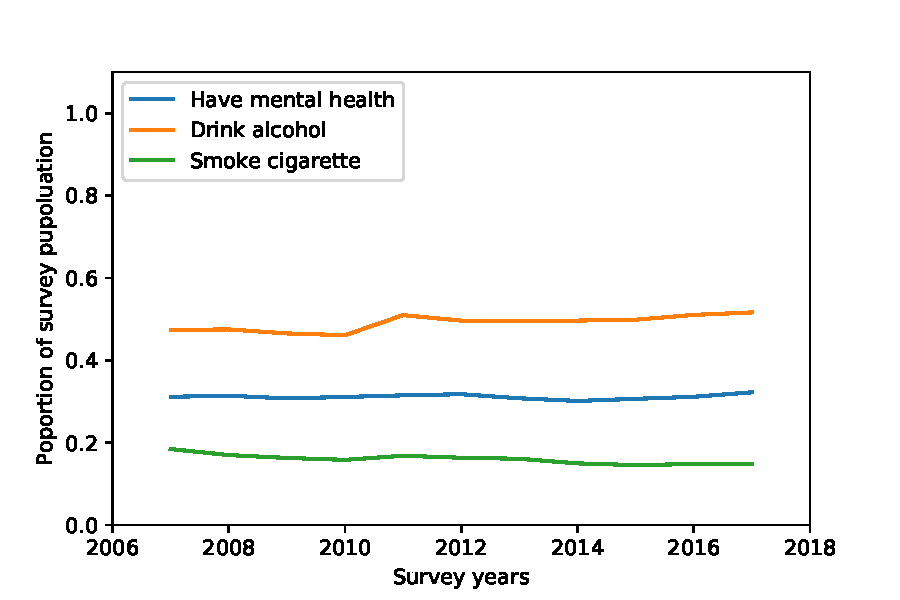
\includegraphics[width=\linewidth]
        {hadi.pdf}}
        \caption{\label{fig:smoke-drink} Smoking and drinking vs. mental issues.}
\end{figure}

With respect to physical activity in Figure \ref{fig:physical}, we compared NOT working out and having mental issues.
The results are stunning. proportion of people from sample population is almost equal to proportion of those do not 
have physical activity. In other words, low physical activity can be directly affecting the mental health and deteriorating it. 

\begin{figure}[!htb]
        \center{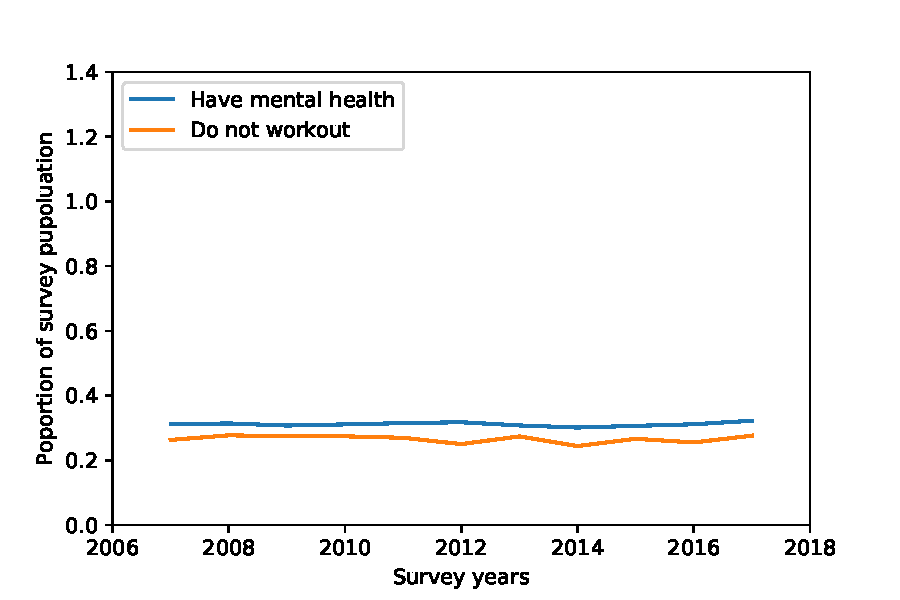
\includegraphics[width=\linewidth]
        {Quang.pdf}}
        \caption{\label{fig:physical} Physical activity vs. mental issues.}
\end{figure}

When it comes to fruit and vegetables, the Figure \ref{fig:veg-fruit} the data shows that vegetable and fruit consumption is high from 2007 to 2017.
There is a very small trend of increasing and we see similar such trend but in decreasing the mental issues. 
Though the data does not show dramatic effect but one cannot help but notice that consuming fruit and vegetables (healthy food)
has a slight effect on reducing mental health.

\begin{figure}[!htb]
        \center{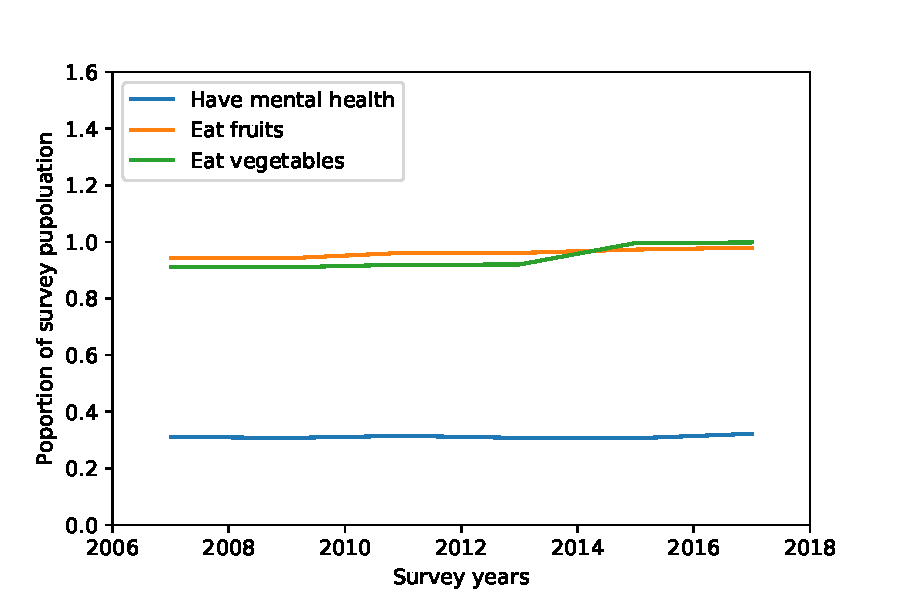
\includegraphics[width=\linewidth]
        {karthik.pdf}}
        \caption{\label{fig:veg-fruit} Eating veggies and fruits vs. mental issues.}
\end{figure}

Using technology (in our case internet) Fig \ref{fig:internt}, on the other hand, shows that increase of usage has increase in mental issues.
The data about internet was available from 2013 and the proportion of sampled population using internet above 70\% and increasing.
We notice that in that period of time (2013-2017), mental issues are increasing.

\begin{figure}[!htb]
        \center{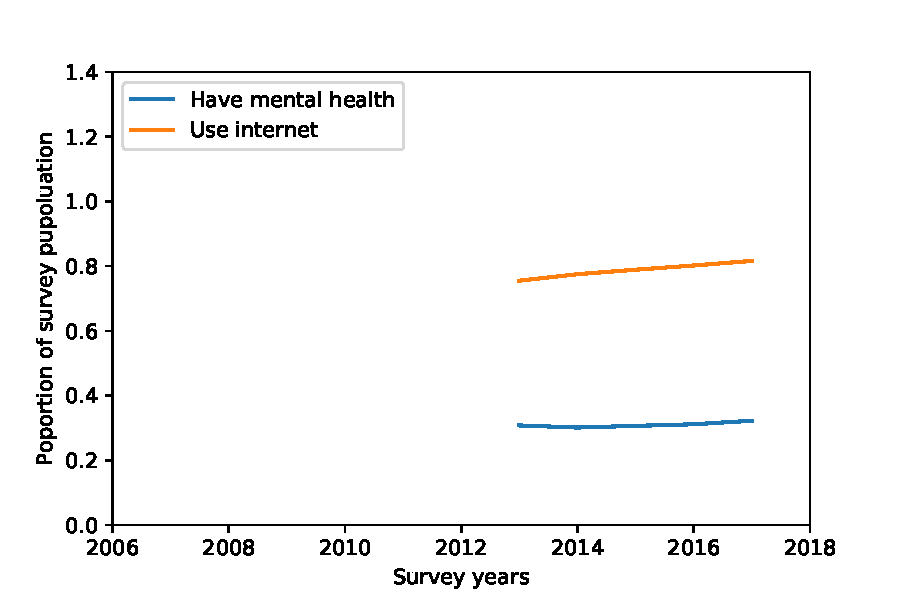
\includegraphics[width=\linewidth]
        {Reza.pdf}}
        \caption{\label{fig:internt} Using internet vs. mental issues.}
\end{figure}

Lastly, Fig \ref{fig:edu} shows that people of the sampled population were almost 90\% had highschool or above degree.
And the number of educators were mildly increasing. We notice that mental issues was decreasing toward last few years and 
it starts to slightly increase. This is very interesting because in our mind, the more you know the better mental health you may have.
Nevertheless, this result does not show it that way. 

We think that education and knowledge would help prevent mental issues but other factors that comes with it, such as using internet, will
offset the good effect of education on mental health and lead to mild increase in the mental issues.

\begin{figure}[!htb]
        \center{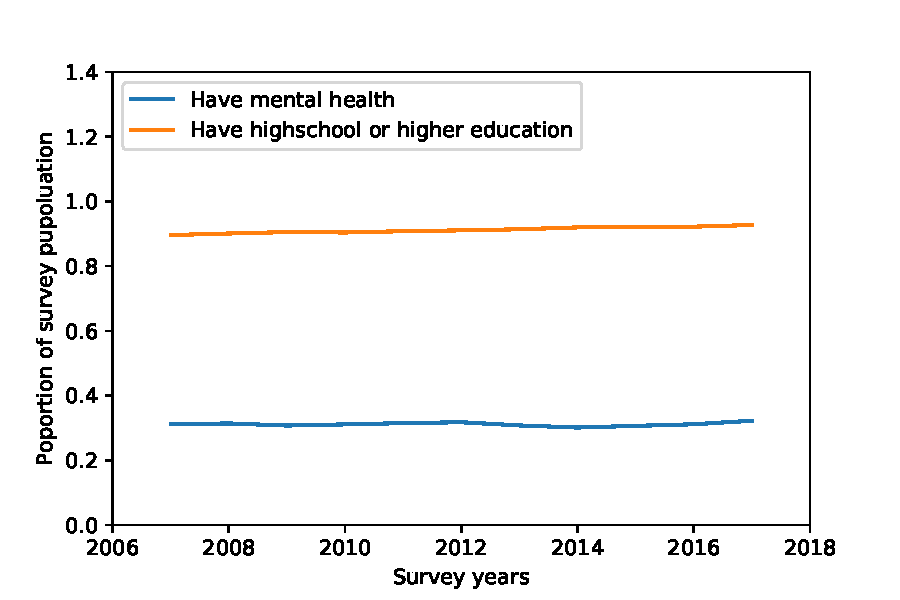
\includegraphics[width=\linewidth]
        {Yuqing.pdf}}
        \caption{\label{fig:edu} Education vs. mental issues.}
\end{figure}

All above mentioned analysis show the results of six factors on US as a whole. We wanted to show the effect more visually and in more details 
for each state.
Therefore, we grouped the data based on year, state, and behavior factor in a website available here \cite{brfss-sqlite}. The visualization
consist of map of united states colored based on the proportion of reported mental health. The higher the mental issue the darker 
the color would show. This an interactive visualization in which user can select a factor, pick a year, and by pointing to each 
state, it provide details of about the that state such as percentage of mental issues and the selected factor reported for that state.
Figure \ref{fig:map} shows one page of this this visualization.  

This visualization provides a summary of the effects of the six factors on each state from year 2007 to 2017. 
By selecting a year, the map extracts data from that year and shows proportion of mental health issues in all states
using the visual choropleth map. Users can visually notice which states reported more mental health issues and by 
hovering the mouse over that state, get the status of picked factor in form of pop up. The visualization is written in D3 \cite{d3} 
and it is portable across all operating systems. The visualization can be publicly reached online \cite{visualization}.

As part of this research, we examined multiple machine learning models to create predictive models for predicting mental health. 
We evaluated six ML models, and examined multiple DL model layer setups.
The accuracy of our models were very low at the beginning. Using hyper-parameters option from scikit-learn \cite{scikit} package, we managed to 
increase the accuracy to 69\%. We also to used DL models for classifications using Keras \cite{keras}. 
Though DL techniques are used in image recognition,
we build a DL classification model and after hours of trainings and neuron layers and density modification, we yet got 68\%.


\begin{figure}[!htb]
        \center{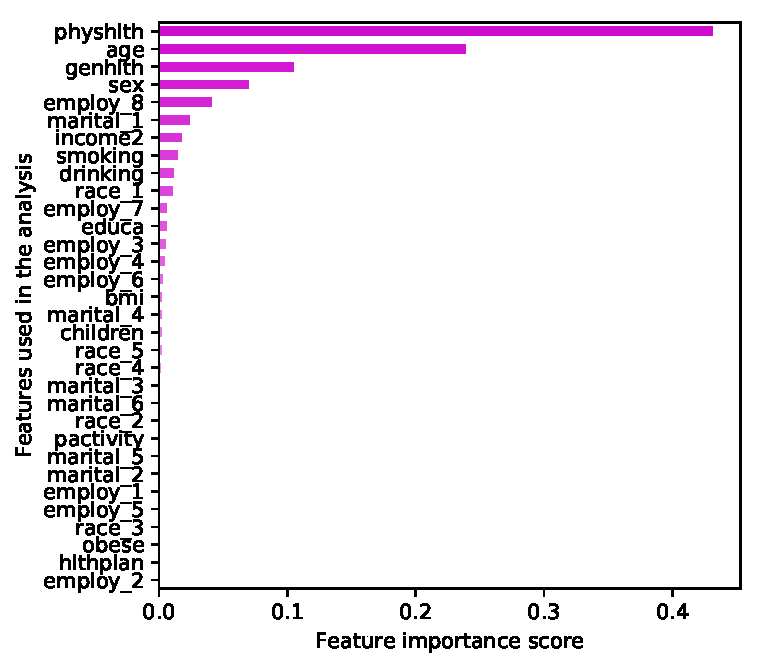
\includegraphics[width=\linewidth]
        {featureImportance2.pdf}}
        \caption{\label{fig:featureImportance} Feature importance.}
\end{figure}

To enhance our analysis, we took our research one step up and re-evaluated features we used in our analysis.
We only focused on Random Forest, Gradient Boosting, and Deep Learning models. 
We added features such as income, general health, details on education, BMI, and few others into 
our model and evaluated the importance of these features. We dropped features that was not present in all years between 2007 and 2017.
We used MinMax to normalize our features and get them between 0 and 1. 
We took logarithm on some feature (such as BMI) to confine their value to 0 and 1.
We applied PCA using the first 24 principle components to capture 97\% variance and to reduce dimensionality of our model for training speedup.
The result of this effort was that the accuracy of our model for both Random Forest and Gradient Boosting increased to 72\%.
Our DL model with the new feature selected, also produced a model with accuracy 72\%. 

\begin{figure}[!htb]
        \center{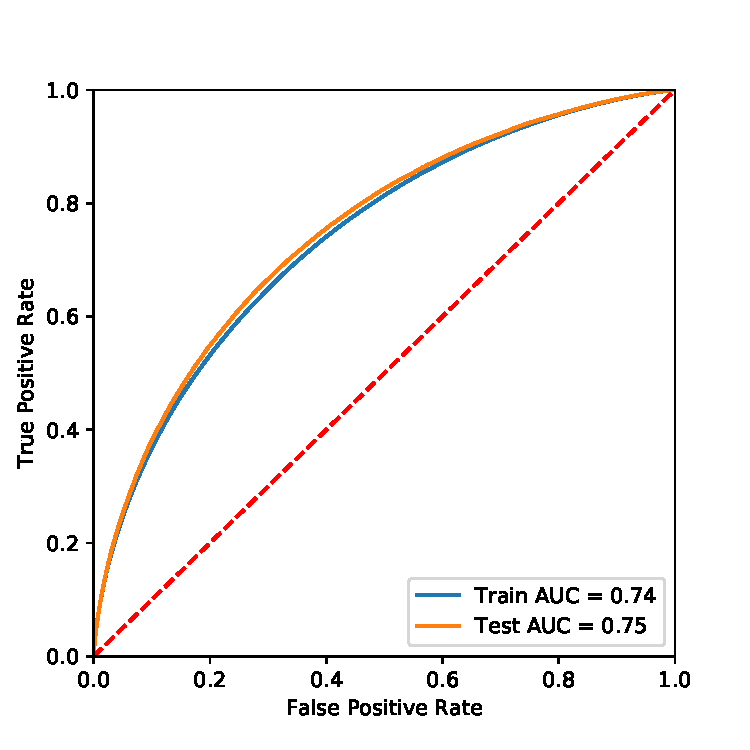
\includegraphics[width=\linewidth]
        {ROC.pdf}}
        \caption{\label{fig:featureImportance} Probability Curve (ROC).}
\end{figure}

Fig \ref{fig:featureImportance} shows feature importance score (between 0 to 0.5) of our models. 
In this figure, the higher a feature score, the more effective a feature is to the model. 
Fig \ref{fig:project-features} shows more details on the features we used for our models. 
The ROC (Receiver Operating Characteristics) curve for train and test data set shows that 
The test AUC (Area Under The Curve) is higher than the train AUC (0.75 vs 0.74) which 
could indicate an underfitting problem. Clearly there is a room for feature selection improvement. 


We are not pleases with this accuracy but not disappointed either. We are planning to put more time and effort
as a follow up on this research to increase the accuracy to above 90\%.  


\section{CONCLUSION AND DISCUSSION}
The research showed that behavioral habits has effect on mental health particularly on depression and anxiety. 
It showed a direct relationship between mental health and the six habit factors. The six factors are: 
smoking, drinking, physical activity, eating disorder (in form of not eating healthy at all), social media (internet), and education.

The research conducted set of analysises to extract the data from BRFSS dataset from 2007 to 2017. The analytics activities included, data conversion, 
cleaning, normalization, aggregation, and applying machine and deep learning algorithms. The best accuracy achieved was 69\% with the 
six features of the research and got enhanced to 72\% after tuning the model by adding new features and removing some features.
The accuracy is not breathtaking but, at this stage of research, is a good starter. The analytics model is based on Random Forest method
for classification and prediction.

The research also produced an interactive visualization that showed the effects of the six factors on mental health in the form of choropleth map
in which user can visually interact with the map and get information on the proportion of BRFSS takers who has mental health and one of the 
six factors for year 2007 to 2017. 

\captionsetup[figure]{labelformat=empty}
\clearpage 
\begin{figure}[hbt!]
        \centering
        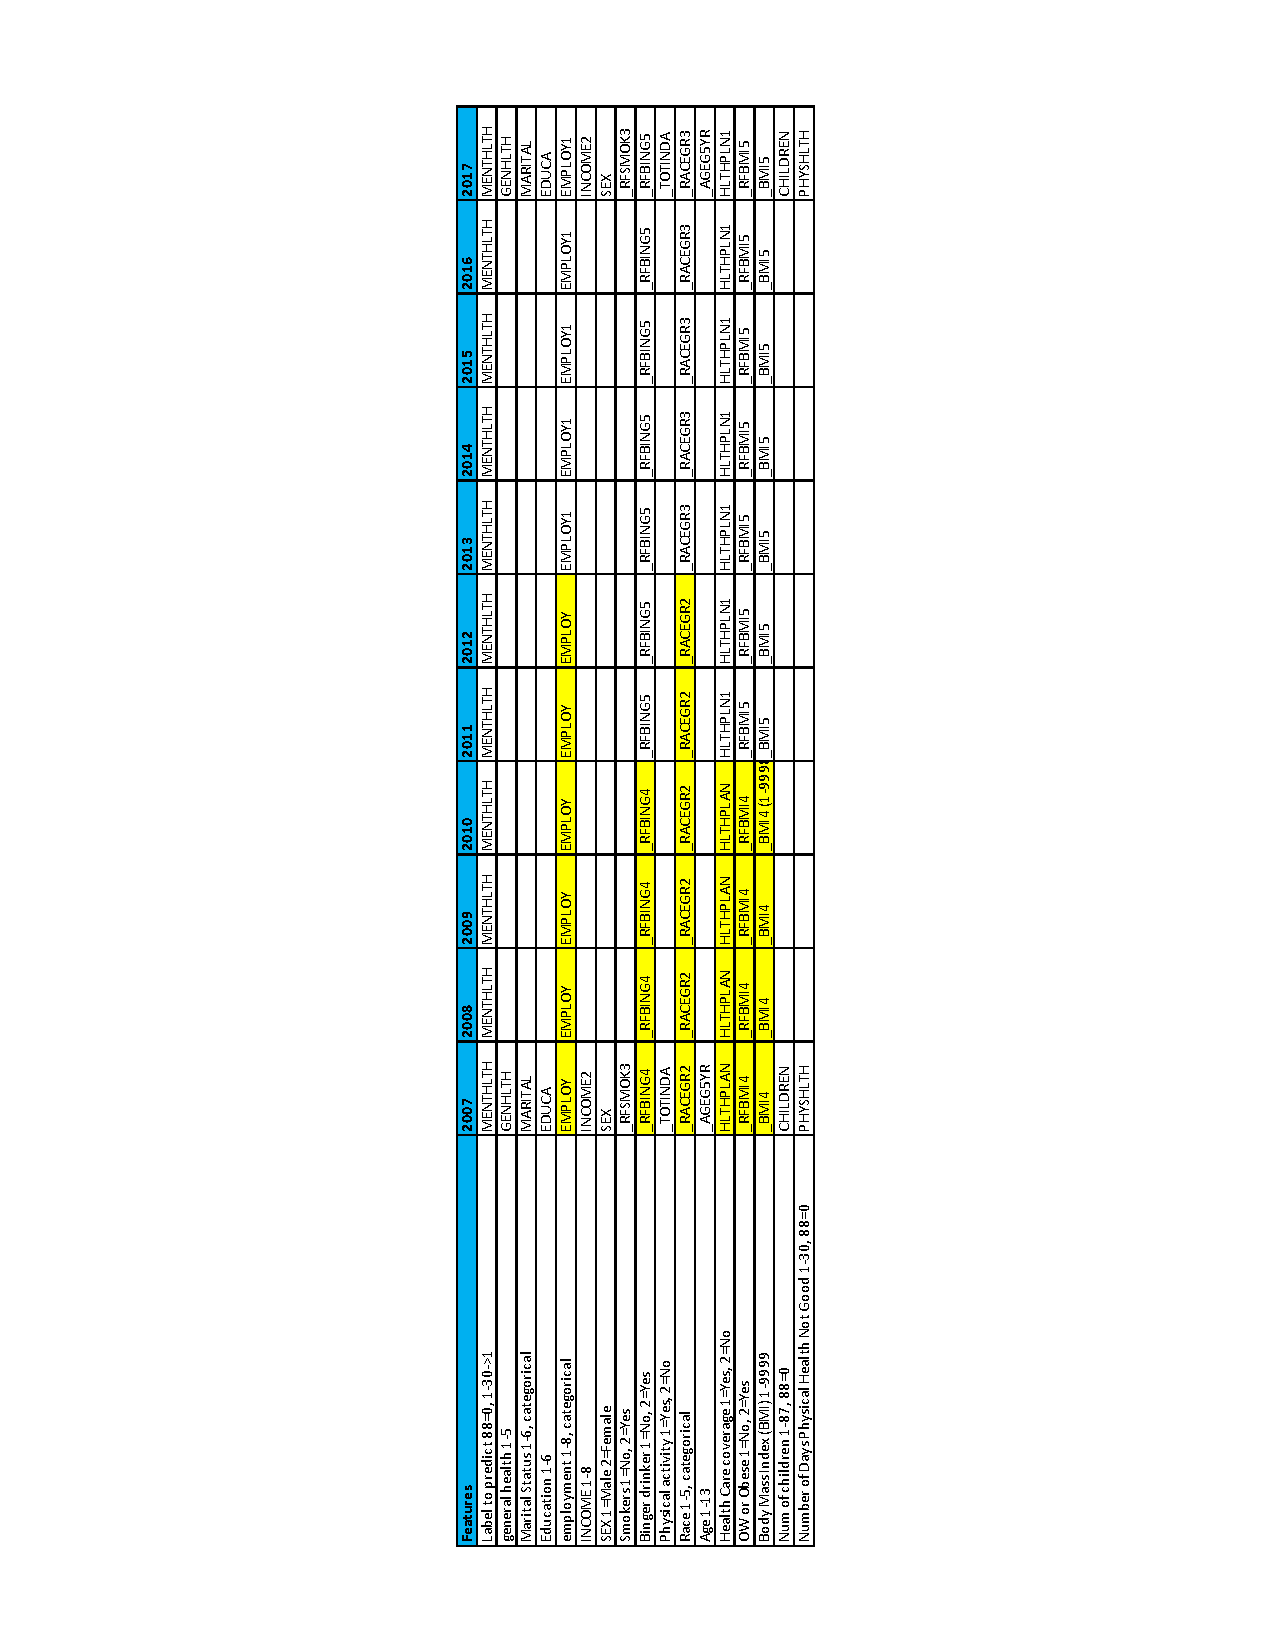
\includepdf[pages=-]{Project_features-rotated.pdf}
        \addvspace{250pt}
        
        \hspace{-10cm}
        \rotatebox{90}{ Figure ~\ref{fig:project-features}: Enhancing the statistical model by tuning features.}
        
        %\caption{The Schedule of all tasks defined for the team.}
        \caption{}
        \label{fig:project-features}
\end{figure}
\clearpage 

\captionsetup[figure]{labelformat=empty}
\clearpage 
\begin{figure}[hbt!]
        \centering
        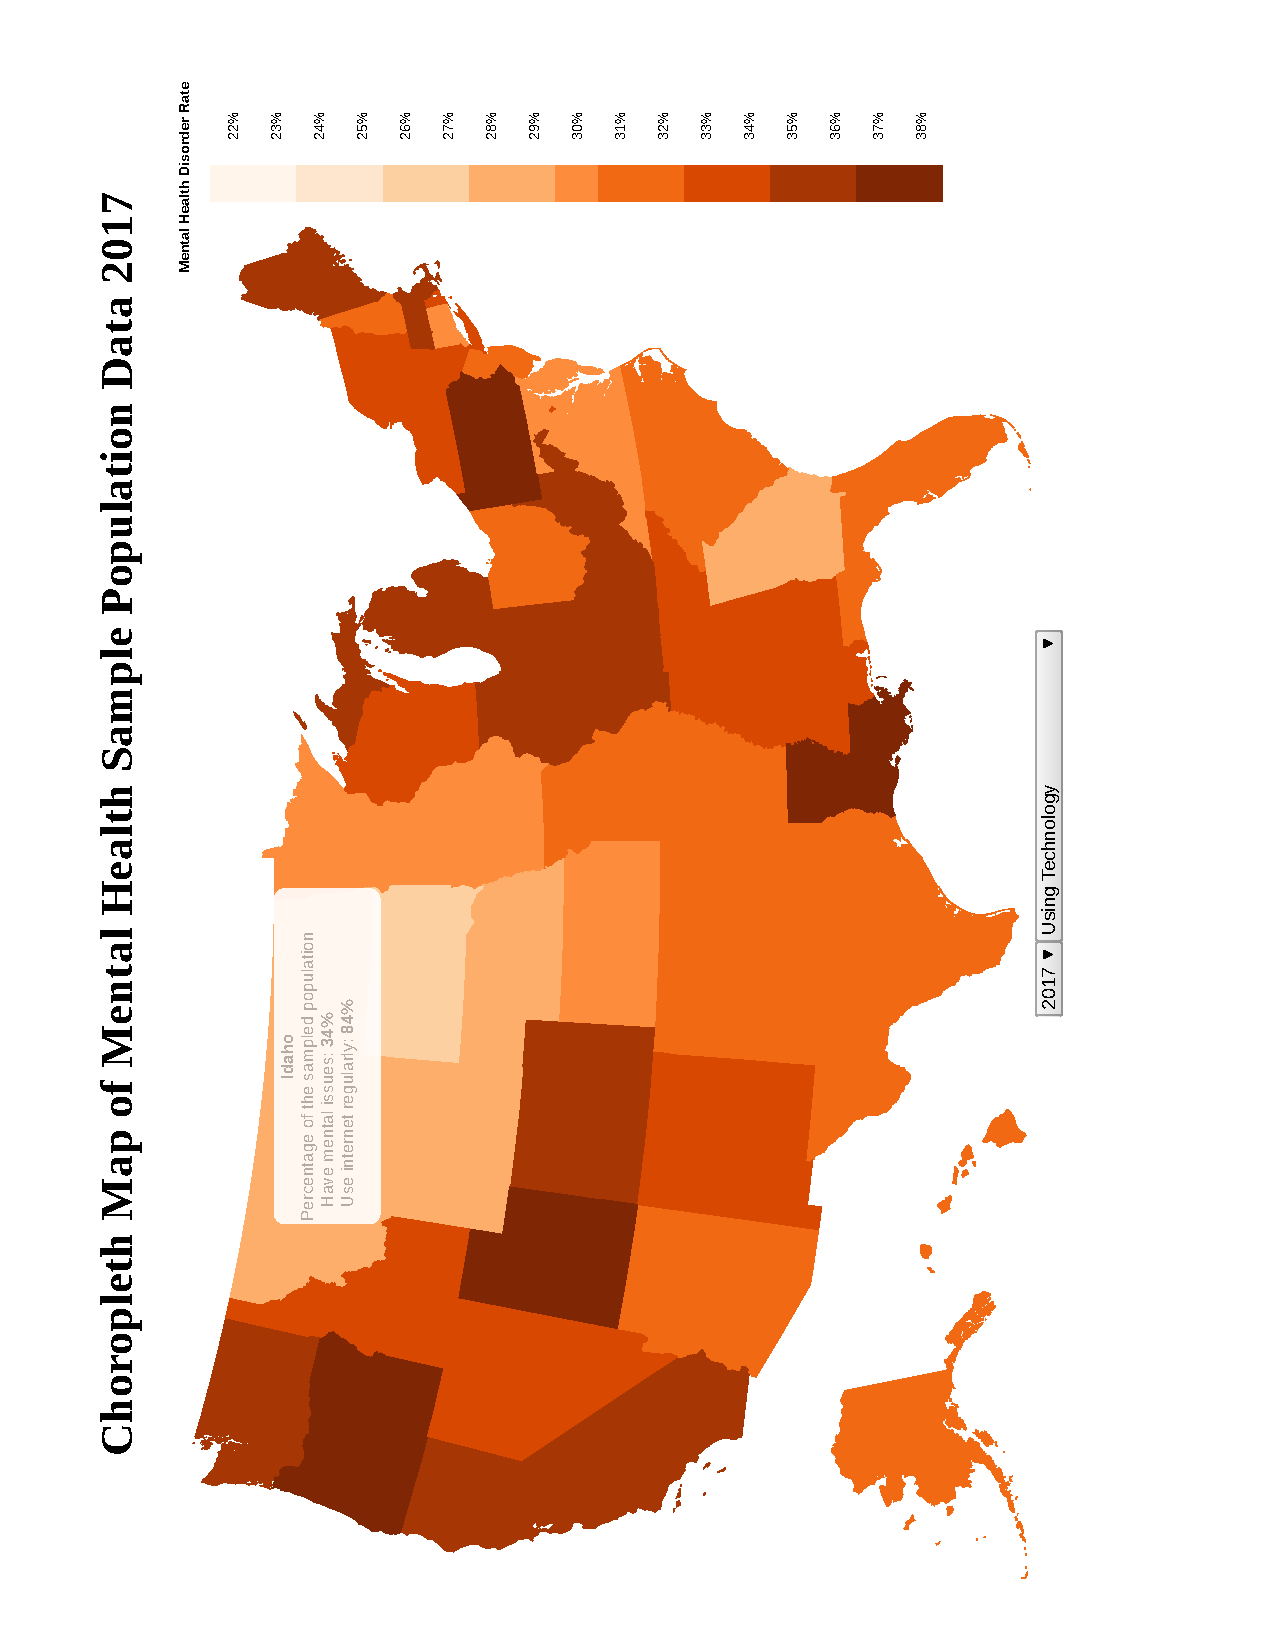
\includepdf[pages=-]{map-rotated.pdf}
        \addvspace{250pt}
        
        \hspace{-10cm}
        \rotatebox{90}{ Figure ~\ref{fig:map}: Six factors vs. mental health for all states.}
        
        %\caption{The Schedule of all tasks defined for the team.}
        \caption{}
        \label{fig:map}
\end{figure}
\clearpage 

\captionsetup[figure]{labelformat=empty}
\clearpage 
\begin{figure}[hbt!]
        \centering
        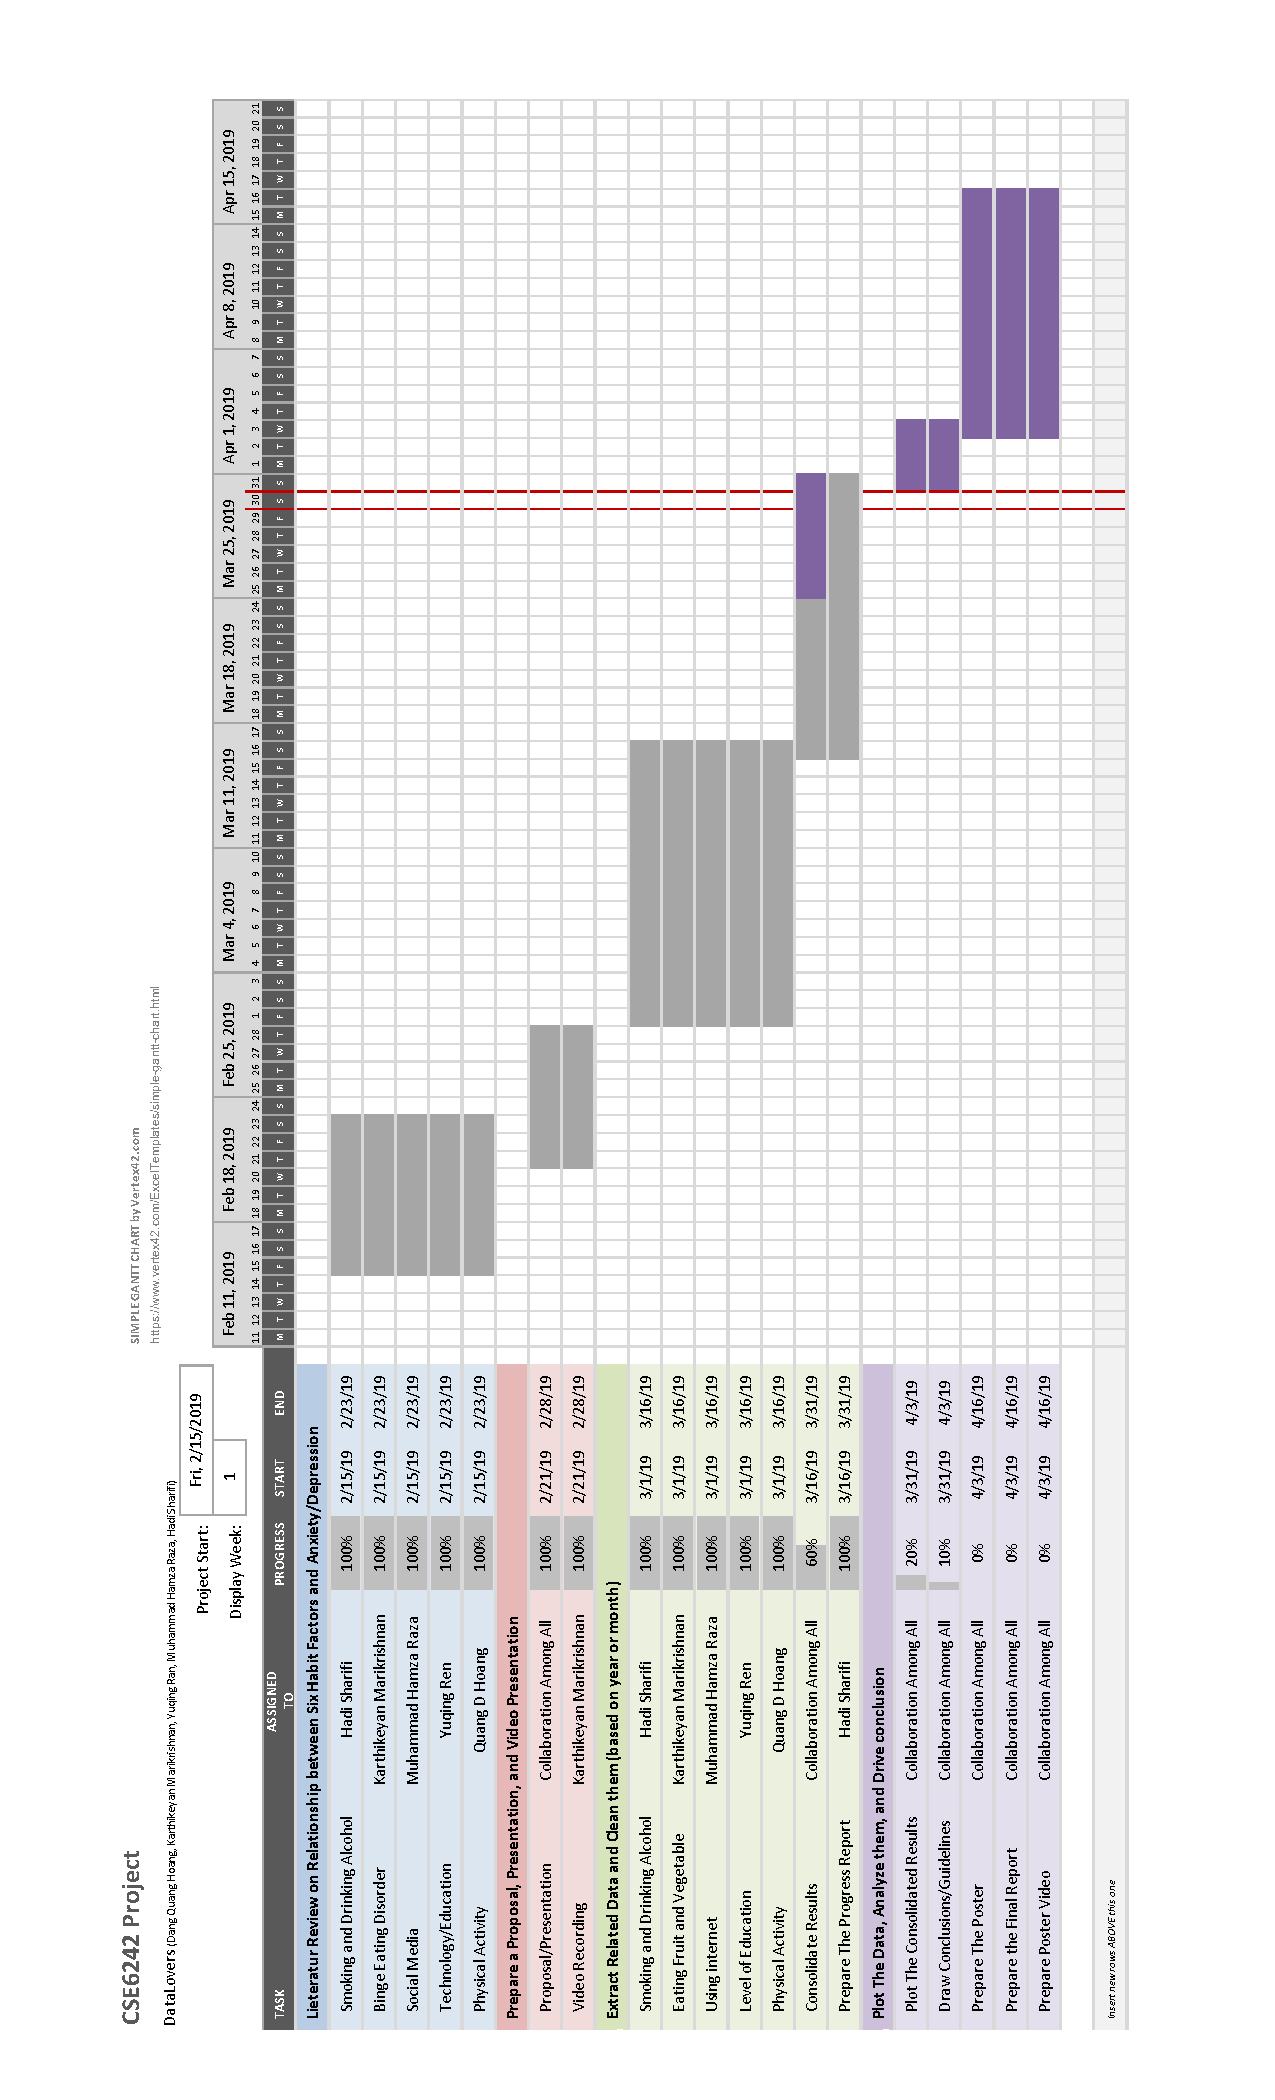
\includepdf[pages=-]{schedule.pdf}
        \addvspace{250pt}
        
        \hspace{-10cm}
        \rotatebox{90}{ Figure ~\ref{fig:schedule}: The schedule of the team for the research.}
        
        %\caption{The Schedule of all tasks defined for the team.}
        \caption{}
        \label{fig:schedule}
\end{figure}

\clearpage 

\bibliography{biblio}
\bibliographystyle{plain}

\section{Appendix}
\begin{figure}[!htb]
        \center{
\includegraphics[width=\linewidth]
        {wordcount.png}}
        \caption{\label{fig:my-label} The total number of words in the report.}
\end{figure}

\end{document}
